\chapter{Boolean Formulas and Equations}
\label{ch:Boolean-Formulas}

Symbolic logic, like other parts of mathematics, starts from a small
collection of axioms and employs rules of inference to find
additional propositions consistent with those axioms. This
chapter will define a grammar of logic formulas, specify a few
equations stating that certain formulas carry the same meaning as others,
and derive new equations
using substitution of equals for equals as the rule of
inference.

You will probably find this familiar from your
experience with numeric algebra, but we will attend carefully
to details, and this formality may extend beyond what you are
accustomed to. What it buys us is mechanization. That is, our
logic formulas and our reasoning about them will amount to
mechanized computation, and this will make it possible to
computers to check that our reasoning follows all the rules,
without exception. This gives us a higher level of confidence
in our conclusions than would otherwise be possible.

\begin{aside}
\emph{Hold on to your seat!} This section illustrates an essential method used throughout the book. It introduces the notion of ``formality'' in mathematical argumentation. This is ``formality'' in the sense of being ``based on formulas.'' The formulas involved have a prescribed grammar similar to the one for numeric formulas that you have used for many years. This grammar is how you know that the formula ``$x+3\times(y + z)$'' is well formed and the non-formula
``$x+3\times(y + ) \times z$'' is not well formed.

Things may seem overly simple at the very beginning. Then, suddenly, you may find yourself thrashing around in deep water. Take a deep breath, and slowly work  through the material.
It provides a basis for everything to follow. It calls for careful study and frequent review when things start to go off track. Fold the corner of this page down. You will probably need to come back to it later.

\caption{Hold on to Your Seat}
\label{aside-hold-on-to-seat}
\end{aside}

We will be doing all of this in the domain of symbolic logic, which
includes operations like ``logical or'' and ``logical negation'',
rather than arithmetic operations, such as addition and
multiplication. Logical operations put our formulas in the
domain of Boolean algebra, rather than numeric algebra, but
our rule of inference, which is substitution of equals for equals,
applies equally well in both the Boolean and the numeric
domains. To illustrate the level of formality that we are
shooting for, let's see how it works with a problem in numeric algebra.

You are surely familiar with the equation $(-1)\times(-1) = 1$, but you may
not know that it is a consequence of some basic facts about
arithmetic calculation. That is, the fact that multiplying two
negative numbers produces a positive one is not independent of
other facts about numbers. Instead, it is an inference one can draw
from an acceptance of other familiar equations.

The equations in Figure~\ref{fig-02-01} (page \pageref{fig-02-01})
express some standard rules of numeric computation. In those equations, the letters stand in
place of numbers, or in place of other
formulas expressed in terms of common numeric operations (addition,
multiplication, etc). We refer to letters used in this way as
``variables'' even though, within a particular equation, they
stand for a fixed number or for a particular formula.
Their values, though unspecific, do not vary.

\begin{figure}
\begin{center}
\begin{tabular}{ll}
$x+0 = x$                & \{$+$ identity\} \\
$(-x)+ x = 0$            & \{$+$ complement\} \\
$x \times 1 = x$         & \{$\times$ identity\} \\
$x \times 0 = 0$         & \{$\times$ null\} \\
$x+y = y+x$              & \{$+$ commutative\} \\
$x+(y+z) = (x+y)+z$      & \{$+$ associative\} \\
$x\times(y+z) = (x \times y)+(x \times z)$      & \{distributive law\} \\
\end{tabular}
\end{center}
\caption{Equations of Numeric Algebra}
\label{fig-02-01}
\end{figure}


If we accept the equations of Figure~\ref{fig-02-01} (page \pageref{fig-02-01}) as axioms,
we can apply one of them to transform the formula $(-1)\times(-1)$ to a new formula that
stands for the same number. Then, we can apply another axiom to
transform that formula to a new one, and so on. We apply the
axiomatic equations in such a way that, at some point, we
arrive at the formula ``1''. At every stage, we know that the
new formula stands for the same value as the old one, so in
the end we know that $(-1)\times(-1) = 1$.

Figure~\ref{fig-02-02} (page \pageref{fig-02-02}) displays this sort of equation-by-equation derivation of the
formula ``1'' from the formula ``$(-1)\times(-1)$''. To
understand Figure~\ref{fig-02-02}, you must remember that each
variable can denote any
grammatically correct formula. For example, in the
\{$+$ identity\} equation, $x + 0 = x$, the variable $x$ could stand for
a number, such as 3, or it could stand for a more complicated
formula, such as $(1 + 3)$. It could even stand for a formula
with variables in it, such as $(a + (b \times c))$ or
$(((-1) \times (x + 3)) + (x + y))$.

Another crucial point is that each step cites
exactly one equation from Figure~\ref{fig-02-01} (page \pageref{fig-02-01})
to justify the transformation from the formula in the previous step. We are so accustomed to calculating numeric formulas that we often combine many basic steps into one. When we reason formally, we must not do this. We must justify each step citing an equation from a list of known equations. In our proof of $(-1)\times(-1) = 1$, we will justify steps by citing equations from Figure~\ref{fig-02-01} and from no other source. We will not skip steps. Think of that as you go through the proof, line by line.

The first step in the proof (Figure~\ref{fig-02-02}, page \pageref{fig-02-02}) uses a version of the
\{$+$ identity\} equation in which the variable $x$ stands for the
formula $((-1)\times(-1))$. The second step reads the \{$+$ complement\}
equation backwards (equations go both ways), and in a form
where the variable $x$ stands for the number 1. And so on. The
transformations, step by step, finally confirm that the two formulas
$(-1)\times(-1)$ and 1 stand for the same number.

Pay particular attention to the last three lines of the proof.
Most people tend to jump from the formula $0+1$ to the formula $1$ in one step. This requires knowing the equation $0+1 = 1$. However, that equation is not among those listed in Figure~\ref{fig-02-01} (page \pageref{fig-02-01}). To do the proof without citing any equations other than those in Figure~\ref{fig-02-01}, we need two steps, and those are the last two steps in the proof.

\begin{figure}
\begin{center}
\begin{tabular}{lll}
    & $(-1)\times(-1)$                            & \\
$=$ & $((-1)\times(-1)) + 0$                      & \{$+$ identity\} \\
$=$ & $((-1)\times(-1)) + ((-1) + 1)$             & \{$+$ complement\} \\
$=$ & $(((-1)\times(-1)) + (-1)) + 1$             & \{$+$ associative\} \\
$=$ & $(((-1)\times(-1)) + ((-1) \times 1)) + 1$  & \{$\times$ identity\} \\
$=$ & $((-1)\times((-1) + 1)) + 1$                & \{distributive law\} \\
$=$ & $((-1)\times 0) + 1$                        & \{$+$ complement\} \\
$=$ & $0 + 1$                                     & \{$\times$ null\} \\
$=$ & $1 + 0$                                     & \{$+$ commutative\} \\
$=$ & $1$                                         & \{$+$ identity\} \\
\end{tabular}
\end{center}
\caption{Why $(-1)\times(-1)=1$}
\label{fig-02-02}
\end{figure}

One of the things we hope you will glean from this derivation is that
the equation $(-1)\times(-1) = 1$ does not depend on vague,
philosophical assertions like ``two negatives make a positive.''
Instead, the equation $(-1)\times(-1) = 1$ is a consequence of some
basic arithmetic equations. If you accept the basic equations
and the idea of substituting equals for equals, you must, as a
rational consequence, accept the equation $(-1)\times(-1) = 1$.

Using this same kind of reasoning, we will derive equations between
formulas in logic from a few, simple equations postulated as
axioms. We will also learn that digital circuits are physical
representations of logic formulas, and we will be able to
parlay this basic idea to derive behavioral properties of
computer components.

Likewise, because a computer program is,
literally, a logic formula, we will be able to derive
properties of those programs directly from the programs,
themselves. This makes it possible for us to be entirely
certain about some of the behavioral characteristics of
software, and of computer hardware, too, since a hardware component is also a logic formula. Our certainty stems from the mechanistic
formalism that we insist on from the beginning,
which can be checked to the last detail with automated computation.

\begin{ExerciseList}
\label{ex:ch02-intro}
\Exercise
Use the equations of Figure~\ref{fig-02-02} (page \pageref{fig-02-02}),
together with the additional equation (1+1)=2, to derive the equation $(x + x) = (2 \times x)$.

\Exercise
Derive the equation $((((-1) \times x) + (2 \times x)) + x) = (2 \times x)$
using using the equations of Figure~\ref{fig-02-02}.

\Exercise
Derive the equation $((x + (((-1) \times (x + y)) + z)) + y) = z$
using using the equations of Figure~\ref{fig-02-02}.
\end{ExerciseList}

\section{Boolean equations}
\label{sec:boolean-equations}
Let's start with the Boolean equations in Figure~\ref{fig-02-03} (page \pageref{fig-02-03}).
If they look strange to you, try not to worry. Everything new seems
strange for a while. Try to view them as ordinary, algebraic
equations, but with a different collection of operators. A
formula in numeric algebra contains operations like addition
($+$) and multiplication ($\times$). Boolean formulas employ logic
operations: logical-and ($\wedge$), logical-or ($\vee$),
logical-negation ($\neg$), and implication ($\rightarrow$).

Furthermore, Boolean formulas stand for logic values
($True$, $False$), rather than for numbers (\dots -1, 0, 1, 2 \dots).
So, in Boolean algebra there are just two basic values ($True$, $False$),
not an infinite collection of numbers.
That does not limit the potential domain of discourse, however. By
aggregating the basic $True$/$False$ elements in sequences, we
will find that we can deal with numbers and with the full range of things that
numbers can represent.

\begin{figure}
\begin{center}
\begin{tabular}{ll}
$x \vee False = x$                                   & \{$\vee$ identity\} \\
$x \vee True = True$                                 & \{$\vee$ null\} \\
$x \vee y = y \vee x$                                & \{$\vee$ commutative\} \\
$x \vee (y \vee z) = (x \vee y) \vee z$              & \{$\vee$ associative\} \\
$x \vee (y \wedge z) = (x \vee y) \wedge (x \vee z)$ & \{$\vee$ distributive\} \\
$x \rightarrow y = (\neg x) \vee y$                  & \{implication\} \\
$\neg(x \vee y) = (\neg x) \wedge (\neg y)$          & \{$\vee$ DeMorgan\} \\
$x \vee x = x$                                       & \{$\vee$ idempotent\} \\
$x \rightarrow x = True$                             & \{self-implication\} \\
$\neg(\neg x)  = x$                                  & \{double negation\} \\
\end{tabular}
\end{center}
\caption{Basic Boolean equations (axioms)}
\label{fig-02-03}
\end{figure}

When we derive new equations from equations we already know,
we refer to the derived equations as ``theorems'' to
distinguish them from axioms. We call the derivation a
``proof'' of the theorem.

The first equation in the
following theorem \{$\vee$ truth table\} is a special case of the
\{$\vee$ identity\} axiom in Figure~\ref{fig-02-03} (see page \pageref{fig-02-03}),
and the proof of that equation consists of that observation. The proof of the
second equation is equally short, but cites
a different equation in the axioms of Figure~\ref{fig-02-03}
to justify the transformation from $False \vee True$
to $True$.
For practice, try to prove the other two
equations in the \{$\vee$ truth table\} theorem by citing axioms
in a similar way.

\label{or-truth-table}
\begin{theorem}[\{$\vee$ truth table\}]
\mbox{}
\begin{itemize}
\item $False \vee False = False$
\item $False \vee True  = True$
\item $True  \vee False = True$
\item $True  \vee True  = True$
\end{itemize}
\end{theorem}

\begin{proof}
\mbox{} \\
\begin{tabular}{llp{3.15in}}
    & $False \vee False$               & \\
$=$ & $False$                          & \{$\vee$ identity\} \dots taking $x$ in the axiom to stand for False \\
\end{tabular}

\begin{tabular}{llp{3.15in}}
    & $False \vee True$                & \\
$=$ & $True$                           & \{$\vee$ null\} \dots taking $x$ in the axiom to stand for False \\
\end{tabular}

\begin{tabular}{lll}
& \dots for practice, prove the other two equations yourself \dots & \\                              & \\
\end{tabular}

\end{proof}

We are serious about that. Did you prove the other two equations?
No? Well \dots go back and do it, then. Without participation, there
is no learning.

Finished now? Good for you. You cited the \{$\vee$ identity\} axiom in your
proof of the third equation in the theorem and the \{$\vee$ null\}
axiom in your proof of the fourth equation, right? We knew you could do it.

\begin{aside}
A ``truth table'' for a formula is a list of the values the formula represents,
with one entry in the list for every possible combination of the values of its variables.
If there is only one variable in the formula, there will be two entries in its truth table,
one for the case when the variable has the value $True$ and one for the case when the variable has the value $False$.
If there are two variables in the formula,
there will be four entries in the truth table because for each choice of value for the first variable,
there are choices for the other. Three variables lead to eight entries.
The number of entries doubles with each new variable.

A truth table for a logical operator is the truth table for the formula that has variables in place of the operands. For example, the truth table for the logical-or operator ($\vee$) is the truth table for the formula $x \vee y$. That formula has two variables, so the truth table has four entries.
\caption{Truth Tables}
\label{truth-tables}
\end{aside}

Derivations are usually more complicated, of course. For example, the following
\{$\vee$ complement\} theorem is not a special case of any
of the axioms, but has a two-step proof, citing implication
and self-implication.

\begin{theorem}[\{$\vee$ complement\}]
$(\neg x) \vee x = True$
\end{theorem}
\begin{proof}
\mbox{}\\
\begin{tabular}{lll}
    & $(\neg x) \vee x$ & \\
$=$ & $x \rightarrow x$ & \{implication\} \\
$=$ & $True$            & \{self-implication\} \\
\end{tabular}

\end{proof}

The \{$\vee$ complement\} theorem is often referred to as the
``law of the excluded middle'' because it states that any
logical statement, together with its negation, comprises all
of the possibilities. A logical statement is either true of false.
There is no middle ground.

All of the logical operators have truth tables, and we can derive the equations in those truth tables from the axioms. The following theorem provides the
truth table for the negation ($(\neg x)$) operator. The proof of the first equation in the \{$\neg$ truth table\} theorem has a four step proof.
To beef up your comprehension of the ideas, construct your own proof of the second equation in the theorem.

\begin{theorem}[\{$\neg$ truth table\}]
\mbox{}\\
\begin{itemize}
\item $\neg True = False$
\item $\neg False = True$
\end{itemize}
\end{theorem}
\begin{proof}
\mbox{} \\
\begin{tabular}{llp{3.15in}}
    & $\neg True$                      & \\
$=$ & $\neg (False \rightarrow False)$ & \{self-implication\} \\
$=$ & $\neg ((\neg False) \vee False)$ & \{implication\} (taking both $x$ and $y$ in the axiom to stand for $False$) \\
$=$ & $\neg (\neg False)$              & \{$\vee$ identity\} (taking $x$ in the axiom to stand for $\neg False$) \\
$=$ & $False$                          & \{double negation\} (taking $x$ in the axiom to stand for False) \\
\end{tabular}

\bigskip
\noindent
\begin{tabular}{lll}
    & $\neg False$                             & \\
$=$ & \dots you fill in the details here \dots & \\
$=$ & $True$                                   & \\
\end{tabular}

\end{proof}

An important facet of these proofs is that they are
entirely syntactic. That is, they apply axioms by
matching the grammar of a formula $f$ in the proof with a formula $g$ in an equation from the axioms.
This matching associates the variables in $g$ with certain sub-formulas in the formula $f$.
Then, the formula $h$ on the other side of
the equation, with the same association between its variables and sub-formulas of $f$,
becomes the new, derived formula.
We know that the derived formula stands for the same value
as the original formula because the axiom asserts this relationship,
and we are assuming that axioms are right.

\begin{aside}
Another way to prove that two formulas stand
for the same value is to build truth tables for both formulas.
A truth table lists all possible combinations of values for the
variables in a formula, and displays the value that the formula
denotes for each of those combinations. (Theorem \{$\vee$ truth table\} provides
the truth table for the logical-or operation, and theorem \{$\neg$ truth table\}
provides the truth table for the logical-negation operation.)
Two truth tables that list identical values of the corresponding
formulas for all combinations of values for
the variables demonstrate that the formulas always stand for the
same value. This proof method works well for formulas with only
a few variables. In that case, there are only a few combinations
of values for the variables, and the comparison can be completed quickly and accurately.

On the other hand, if there are many variables in the formulas,
things get out of hand. With two variables, as in the truth table
for logical-or, there are four combinations of values
(two choices for each variable, $True$ or $False$, so two times two
combinations in all). With three variables, there are eight
($2^3$) combinations, which makes the truth-table method tedious,
but not infeasible. After that, it gets rapidly out of hand.
Ten variables produce 1,024 ($2^{10}$) combinations of values.
That makes it difficult for people, but no real problem for a computer.
Even twenty variables (a little more than a million combinations)
also can be checked quickly by computers.

However, the formula specifying a computing component,
hardware or software, has hundreds of variables.
Our goal is to be able to reason about
computing components, and there is no hope of doing
that when the formulas have hundreds of variables. The number of combinations
of values for the variables in a formula with, say,
100 variables is $2^{100}$, and that number is so large that no computer could
finish checking for equality before the sun runs out of fuel.

So, it is definitely not feasible to know the full meaning
of computing components by analyzing the truth tables of the
formulas that comprise their designs. Reasoning based on grammatical form
makes it feasible to deal with realistic computing components
because the reasoning process can be split into parts small enough
to manage, and those parts can be reintegrated, based on
their grammatical relationships, to produce a full analysis.
It will take some diligence to reach this goal, and
we will need a few more tools, but the proof methods
of this chapter will get us started in the right direction.
\caption{Truth Tables and Feasibility}
\label{feasibility}
\end{aside}

Let's do another truth-table theorem, partly to practice
reasoning with equations, but also to discuss a common
point of confusion about logic. The implication operator
($\rightarrow$) is a cornerstone of logic in real-world problems,
but many people misunderstand its meaning (that is, its truth table).

The \{$\rightarrow$ truth table\} theorem provides the truth table for the implication operator. An important aspect of the proof is that it cites not only axioms from Figure~\ref{fig-02-03} (see page \pageref{fig-02-03}),
but also equations from the \{$\neg$ truth table\} theorem. This is the way mathematics goes. Once we have derived a new equation from the axioms, we can cite the new equation to derive still more equations.

\begin{aside}
 Citing proven theorems to prove new ones is similar to an idea known as ``abstraction''
 that is a mainstay in engineering design.
 At the point where we cite an old theorem to prove a new one,
 we could, instead, copy the proof of the old theorem into new proof.
 However, that would make the proof longer, harder to understand,
 and more likely to contain errors.

 Computer programs are built from components that are, themselves, other computer programs. As the project proceeds, more and more components become available, and they are used to build more complex ones. Sometimes, a component has almost the right form to be used in a new program, but not quite. Maybe the existing component doubles a number where the new program would need to triple it. Most software engineers are tempted to make a copy the old component and change the $2 \times x$ formula to $3 \times x$ at the point where a doubling should be a tripling. \emph{This practice the single most common cause of errors in computer software.}

 What the engineer should do is to make a new component in which the $2$ is replaced by a variable, say $m$. This is known as creating an ``abstraction'' of the component (``abstract'' as opposed to ``specific'' or ``concrete''). The new component can be used for both doubling and tripling, simply by specifying $2$ for $m$ in one case and $3$ for $m$ in the other. That way, if the component turns out later to have an error in it, the error can be fixed in one place instead of two (or maybe ten or a hundred places, depending on how many engineers have made copies of the original component to change the $2$ to $7$ or $9$ or whatever.

Abstraction is one of the most important methods in all of engineering design. Citing old theorems to prove new ones, instead of copying their proofs into the new proof with appropriate choices for the variables, is part of that tradition.

\caption{Abstraction}
\label{abstraction}
\end{aside}

\begin{theorem}[\{$\rightarrow$ truth table\}]
\label{implication-truth-table}
\mbox{}
\begin{itemize}
\item $False \rightarrow False = True$
\item $False \rightarrow True  = True$
\item $True  \rightarrow False = False$
\item $True  \rightarrow True  = True$
\end{itemize}
\end{theorem}

\begin{proof}
\mbox{} \\
\begin{tabular}{llp{3.15in}}
    & $False \rightarrow False$        & \\
$=$ & $(\neg False) \vee False$        & \{implication\} \dots taking both $x$ and $y$ in the axiom to stand for $False$ \\
$=$ & $\neg False$                     & \{$\vee$ identity\}\\
$=$ & $True$                           & \{$\neg$ truth table\}\\
\end{tabular}

\begin{tabular}{lll}
& \dots for practice, prove the other equations yourself\dots & \\         & \\
\end{tabular}

\end{proof}

In day to day life outside the sphere of symbolic logic,
the interpretation of the logical implication ``$x \rightarrow y$''
is that we can conclude that $y$ is true if we know that
$x$ is true. However, the implication says nothing
about $y$ when $x$ is not true. In particular, it
does not say that $y$ is not true whenever $x$ is not true.
A quick look at theorem \{$\rightarrow$ truth table\} shows that the
formula ``$False \rightarrow y$'' has the value $True$ when $y$ is $True$
and also when $y$ is $False$.
In other words, the truth of the formula $x \rightarrow y$ in the case
where the hypothesis, $x$, of the implication is $False$ provides
no information about the conclusion, $y$.

A common mistake in everyday life is to assume that if the
implication ``$x \rightarrow y$'' is true, then the implication
``$(\neg x) \rightarrow (\neg y)$''
is also true. Sometimes this leads to bad
results, even in everyday life. In symbolic logic,
it is worse than that. Such a conclusion puts an
inconsistency into the mathematical system, and that renders the system useless.

Over half of the basic Boolean equations in Figure~\ref{fig-02-03} (see page \pageref{fig-02-03})
have names associated with the logical-or ($\vee$) operation.
One of them, the
\{$\vee$ DeMorgan\} equation establishes a connection between logical-or and logical-and.
It converts the negation of a logical-or to the logical-and of two negations:
$\neg(x \vee y) = (\neg x) \wedge (\neg y)$.
We can use this connection to prove a collection of equations for logical-and that are similar to the basic ones for logical-or.
An example is the null law for logical-and.

\begin{theorem}[\{$\wedge$ null\}]
$x \wedge False = False$
\end{theorem}

\begin{proof}
\mbox{} \\
\begin{tabular}{llp{3.15in}}
    & $x \wedge False$                       & \\
$=$ & $x \wedge (\neg True)$                 & \{$\neg$ truth table\} \\
$=$ & $(\neg (\neg x)) \wedge (\neg True)$   & \{double negation\} \\
$=$ & $\neg ((\neg x) \vee True)$            & \{$\vee$ DeMorgan\} \dots taking $x$ in the axiom to stand for $(\neg x)$ and $y$ in the axiom to stand for $True$  \\
$=$ & $\neg True$                            & \{$\vee$ null\} \\
$=$ & $False$                                & \{$\neg$ truth table\} \\
\end{tabular}

\end{proof}

This regime of theorem after theorem, proof after proof, is a little tiresome, isn't it?
Nevertheless, let's push through one more.
Then we'll give you a few to work out on your own, and go on to other topics.
We're not abandoning proofs, though. Just taking a little break.
It's going to be one proof after another, all the way down the line.

Some equations simplify the target formula when used in one direction,
but make it more complicated when used in the other direction.
For example, applying
the null law for logical-or, \{$\vee$ null\}, from left to right simplifies a logical-or formula to $True$.
The formula on the right in the \{$\wedge$ null\} equation discards both the logical-or operation and the variable $x$.
When you use this equation in the other direction, you can make the formula as complicated as you like because the variable $x$ stands for any formula you want to make up (as long as it's grammatically correct).
It can have hundreds of variables and thousands operations.
This may seem perverse, but if that's what it takes to complete the proof, so be it.

The null law for logical-and, \{$\wedge$ null\}, is also asymmetric. It goes from complicated to simple in one direction and from simple to complicated in the other. A particularly interesting and important asymmetric equation is the absorption law for logical-and. It has two variables and two operations on one side, but only one variable and no operations on the other.

\begin{theorem}[\{$\wedge$ absorption\}]
$(x \vee y) \wedge y = y$
\label{and-absorption-thm}
\end{theorem}

\begin{proof}
\mbox{} \\
\begin{tabular}{llp{3.15in}}
    &$(x \vee y) \wedge y$                 & \\
$=$ & $(x \vee y) \wedge (y \vee False)$   & \{$\vee$ identity\} \\
$=$ & $(y \vee x) \wedge (y \vee False)$   & \{$\vee$ commutative\} \\
$=$ & $y \vee (x \wedge False)$            & \{$\vee$ distrubutive\} \\
$=$ & $y \vee False$                       & \{$\wedge$ null\} \\
$=$ & $y$                                  & \{$\vee$ identity\} \\
\end{tabular}

\end{proof}

We hope the gauntlet of theorems and proofs we have run you through (or, more likely, asked you to plow through, to the point of exhaustion) helps you understand how to derive a new equation from equations you already know. The technique requires matching the formula to one side of a known equation, then replacing it by the corresponding formula on the other side.

The ``matching'' process is a crucial step. It involves replacing the variables in the known equation by constituents of the formula you are trying to match. This is based in the mechanics of a formal grammar. It is surprisingly easy to have a lapse of concentration and make a mistake.

Fortunately, it is easy for computers to verify correct matchings and report erroneous ones. A computer system that does this is called a ``mechanized logic.'' After you have enough practice to have a firm grasp on the process, we will begin to use a mechanized logic to make sure our reasoning is correct.

\begin{ExerciseList}
\Exercise
Use the equations of Figure~\ref{fig-02-02} (page \pageref{fig-02-02})
and the $\wedge$-absorption theorem (page \pageref{and-absorption-thm}),
to derive the $\vee$-absorption equation: $(x \wedge y) \vee y = y$.

\Exercise
Derive the equation
$(((\neg x) \wedge b) \vee (a \wedge (\neg b))) = ((a \vee b) \wedge (\neg(a \wedge b))))$
from the equations of Figure~\ref{fig-02-02}.

\Exercise
Derive the equation
$(((\neg x) \wedge b) \vee (a \wedge (\neg b))) = ((a \rightarrow b) \wedge (b \rightarrow a))$
from the equations of Figure~\ref{fig-02-02}.

\Exercise
Use the equations of Figure~\ref{fig-02-02} (page \pageref{fig-02-02})
and the theorems of this section to
derive the truth-table for the following formula $(x \vee ((\neg y) \wedge (\neg z)))$.
\emph{Note}: Since there are three variables in the formula, the truth table
will have eight entries, and you will need to prove eight equations.
Each equation will have on the left-hand side
a different combination of $True$/$False$ values for the variables $x$, $y$, and $z$,
and on the right-hand side will have the appropriate $True$/$False$ value for the formula.
\end{ExerciseList}

\section{Boolean formulas}
\label{sec:boolean-formuas}

We have been doing proofs based on the grammatical elements of formulas, but instead of taking the time to put together a precise definition of that grammar, we have been relying on your experience with formulas of numeric algebra, such as $2(x + y) + 3z$. Surely it would be better to have a precise definition, so we can determine whether or not a formula is grammatically correct. We are going to define a grammar by starting with the most basic elements, and working up from there to more complicated ones.

The simplest Boolean formulas are the basic constants ($True$ and $False$) and variables. We normally use ordinary, lower-case letters, such as $x$ and $y$ for variables. Sometimes variables are letters with subscripts, such as $x_3$, $y_i$, or $z_n$. This gives us sufficient variety for all of the situations we will encounter, but we will assume there is an infinite pool of names for variables. If we run out of Roman letters, we can use Greek letters. If we run out of those, we can start making up recognizable squiggles like Dr Seuss did in some of his stories.

So, if you write $True$, or $False$, or a lower-case letter, you have composed a grammatically correct Boolean formula. This is the first rule of Boolean grammar. Formulas conforming to this rule have no substructure, so we call them ``atomic'' formulas.

To make more complicated formulas, we use Boolean operators. We refer to the operators that require two operands as the ``binary operators'' ($\wedge$, $\vee$, and $\rightarrow$). These operators lead to the second rule of Boolean grammar: If $a$ and $b$ are grammatically correct Boolean formulas, and $\circ$ is a binary operator (that is, $\circ$ is one of the symbols $\wedge$, $\vee$, or $\rightarrow$), then $(a \circ b)$ is also a grammatically correct Boolean formula.

For example, the first rule confirms that $x$ and $True$ are grammatically correct Boolean formulas. Since $\wedge$ is a binary operator, $(x \wedge True)$ is a grammatically correct Boolean formula by the second rule of grammar. Furthermore, since $\rightarrow$ is a binary operator, and $y$ is a grammatically correct Boolean formula (by the first rule), $((x \wedge True) \rightarrow y)$ must be a grammatically correct Boolean formula (by the second rule). As you can see, the first two rules of Boolean grammar lead to an infinite variety of grammatically correct Boolean formulas.

The third rule of Boolean grammar shows how to incorporate the negation operator in formulas. The rule is that if $a$ is a grammatically correct Boolean formula, then so is $(\neg a)$.

These three rules cover the full range of grammatically correct Boolean formulas, but there is a fine point to discuss about parentheses. Parentheses are important because they make it easy to define the grammar and to explain the meaning of grammatically correct formulas.

The formulas covered by the three rules are fully parenthesized, including a top level of parentheses enclosing the entire formula. Top level parentheses are often omitted in informal presentations, and we have been omitting them on a regular basis.

For example, we have been writing formulas like ``$x \vee y$'', even though they do not have the top-level parentheses required in the grammar of binary operations. To conform to the grammar, we would have to write the formula with its top-level parentheses: $(x \vee y)$. Because we have often omitted top-level parentheses, requiring them probably comes as a surprise. But, allowing non-atomic formulas without top-level parentheses requires additional rules of grammar, and the extra complexity is not compensated by added value.

Here is less a surprising example of incorrect grammar: $x \wedge y \vee z$. This formula is missing two levels of parentheses. Even worse, there are two options for the inner parentheses. Does $x \wedge y \vee z$ mean $((x \wedge y) \vee z)$ or $(x \wedge (y \vee z))$? There is a way to deal with formulas that omit some of the parentheses, but to avoid confusion, we are not going to allow such formulas. The same problem occurs with formulas in numeric algebra. We know that $x \times y + z$ means $((x \times y) + z)$ and not $(x \times (y + z))$ because we know the convention that gives multiplicative operations a higher precedence than additive operations. But that gets some getting used to, and since Boolean formulas may be new to you, we want to minimize the possibility of misinterpretation.

We will sometimes be informal enough to omit the top level of parentheses around the whole formula, but we will not omit any interior parentheses.
We will, however, allow redundant parentheses in grammatically correct formulas. For example, the formula $(x \vee ((x \wedge y)))$ is grammatically correct and has the same meaning as the formula $(x \vee (x \wedge y))$. The first formula has redundant parentheses, but the second one doesn't.
Allowing redundant parentheses requires a fourth rule of grammar:
If $a$ is a grammatically correct Boolean formula, then so is $(a)$.

\begin{figure}
\begin{center}
\begin{tabular}{llll}
$v$             & \{atomic\}    &~~~~& \\
$(a \circ b)$   & \{bin-op\}    &~~~~& \emph{all grammatically correct formulas} \\
$(\neg a)$      & \{negation\}  &~~~~& \emph{~~~must match one of these templates}  \\
$(a)$           & \{group\}     &~~~~& \\
\end{tabular}

\vspace{2 mm}

\emph{requirements on symbols}

\begin{tabular}{l}
\hline
$\bullet$ ~~ $v$ is a variable or $True$ or $False$ \\
~~~~~(a variable is a letter or a letter with a subscript) \\
$\bullet$ ~~ $a$ and $b$ are grammatically correct Boolean formulas \\
$\bullet$ ~~ $\circ$ is a binary operator \\
\hline
\end{tabular}
\end{center}
\caption{Rules of Grammar for Boolean Formulas}
\label{fig-02-grammar}
\end{figure}

With the four rules of Figure~\ref{fig-02-grammar} (see page \pageref{fig-02-grammar}),
we can determine whether or not any given sequence of symbols is a grammatically correct Boolean formula.
The definition of the grammar is circular, but in a useful way that shows how to build more complicated formulas from simpler ones.

To verify that a formula is grammatically correct, find the rule of grammar that matches it, then verify that each part of the formula that matches with a letter in the rule of grammar is also grammatically correct. Atomic formulas have no substructure, so they require no further verification. A line of verification terminates when it arrives at an atomic formula.

For example, consider the formula $((x \vee (\neg y)) \wedge (x \rightarrow z))$. It matches with the \{bin-op\} rule. The symbols in the rule match with the elements of the formula in the following way.
\begin{center}
\begin{tabular}{ll}
\emph{symbol from \{bin-op\} rule}      & \emph{matching element in} $((x \vee (\neg y)) \wedge (x \rightarrow z))$ \\
$a$                                     & $(x \vee (\neg y))$ \\
$\circ$                                 & $\wedge$ \\
$b$                                     & $(x \rightarrow z)$ \\
\end{tabular}
\end{center}

The only other symbols in the rule are the top-level parentheses, and these match identically with the outer parentheses in the target formula. Therefore, the target formula is grammatically correct if the formulas $(x \vee (\neg y))$ and $(x \rightarrow z)$  are grammatically correct. We use the same approach to verify the grammatical correctness of those formulas.

The first one, $(x \vee (\neg y))$, again matches with the \{bin-op\} rule, but this time the matchings of the elements in the target formula with symbols in the rule are as follows:
\begin{center}
\begin{tabular}{ll}
\emph{symbol from \{bin-op\} rule}      & \emph{matching element in}  $(x \vee (\neg y))$ \\
$a$                                     & $x$ \\
$\circ$                                 & $\vee$ \\
$b$                                     & $(\neg y)$ \\
\end{tabular}
\end{center}

This reduces the verification of the grammatical correctness of $(x \vee (\neg y))$ to the verification of the two formulas $x$ and $(\neg y)$. Since $x$ matches with the \{atomic\} rule, it must be grammatically correct. The $(\neg y)$ element matches with the \{negation\} rule, with $y$ from the formula matching $a$ in the rule. So, $(\neg y)$ is grammatically correct if $y$ is, and $y$ is grammatically correct because it matches with the \{atomic\} rule. That completes the verification of the $(x \vee (\neg y))$ formula.

The second element of the original formula, $(x \rightarrow z)$, is easier to verify. It matches the \{bin-op\} rule with $x$ corresponding to $a$ in the rule, $y$ corresponding to $b$, and $\rightarrow$ corresponding to $\circ$ in the rule. Since $x$ and $z$ match the \{atomic\} rule, they are grammatically correct. This completes the verification of the grammatical correctness of the formula $((x \vee (\neg y)) \wedge (x \rightarrow z))$.

Let's look at another example: $(x \vee (\wedge y)$. This formula matches with the \{bin-op\} rule, with $x$ corresponding to $a$ in the rule, $\vee$ corresponding to $\circ$, and $(\wedge y)$ corresponding to $b$. So, the formula is grammatically correct if $x$ and $(\wedge y)$ are. However, there is no rule that matches $(\wedge y)$. The only place the symbol $\wedge$ could match a rule in the table is in the \{bin-op\} rule. In the \{bin-op\} rule, there must be a grammatically correct formula between the opening parenthesis and the operator. Since there is no such element present between the opening parenthesis and the $\wedge$ operator in the target formula, it cannot be grammatically correct.

That covers the grammar of Boolean formulas. What about meaning? Every grammatically correct Boolean formula denotes, in the end, either the constant $True$ or the constant $False$. To find out which, you only need to know which value ($True$ or $False$) each of the variables in the formula stands for. Each of the binary operators, given specific operands ($True$ or $False$), delivers a specific result ($True$ or $False$). We worked out what the delivered values would be for some of the operators when we proved truth-table theorems for them (see page \pageref{or-truth-table}).

In the process of deriving the truth tables,
we used the Boolean equations of Figure~\ref{fig-02-03} (see page \pageref{fig-02-03}).
We can use this same method to derive the meaning ($True$ or $False$) of any grammatically correct formula that contains no variables. However, to deal with parentheses in a completely mechanized way, we need to add two equations to those of Figure~\ref{fig-02-03}. Figure~\ref{fig-02-boolean-axioms} (see page \pageref{fig-02-boolean-axioms})
provides all of the information needed to determine the $True$/$False$ value of any grammatically correct formula that contains no variables. In fact it has even more general applicability. It provides all the information needed to verify not only whether a given formula has the same meaning as the formula $True$ or the formula $False$, but also to verify whether or not any two given, grammatically correct, formulas have the same meaning.

\begin{figure}
\begin{center}
\begin{tabular}{ll}
$(a \vee False) = a$                                     & \{$\vee$ identity\} \\
$(x \vee True) = True$                                   & \{$\vee$ null\} \\
$(a \vee b) = (b \vee a$)                                & \{$\vee$ commutative\} \\
$(a \vee (b \vee c)) = ((a \vee b) \vee c)$              & \{$\vee$ associative\} \\
$(a \vee (b \wedge c)) = ((a \vee b) \wedge (a \vee c))$ & \{$\vee$ distributive\} \\
$(a \rightarrow b) = ((\neg a) \vee b)$                  & \{implication\} \\
$(\neg(a \vee b)) = ((\neg a) \wedge (\neg b))$          & \{$\vee$ DeMorgan\} \\
$(a \vee a) = a$                                         & \{$\vee$ idempotent\} \\
$(a \rightarrow a) = True$                               & \{self-implication\} \\
$(\neg(\neg a))  = a$                                    & \{double negation\} \\
$((a)) = (a)$                                            & \{redundant grouping\} \\
$(v) = v$                                                & \{atomic release\} \\
\end{tabular}

\vspace{2 mm}

\emph{requirements on symbols}

\begin{tabular}{l}
\hline
$\bullet$ ~~ $a$, $b$, and $c$ are grammatically correct Boolean formulas \\
$\bullet$ ~~ $v$ is a variable or $True$ or $False$ \\
~~~~~(a variable is a letter or a letter with a subscript) \\
\hline
\end{tabular}
\end{center}
\caption{Axioms of Boolean Algebra}
\label{fig-02-boolean-axioms}
\end{figure}

\begin{ExerciseList}

\Exercise Use the rules of grammar for Boolean formulas (Figure~\ref{fig-02-grammar}, page \pageref{fig-02-grammar})
to determine which of the following formulas are grammatically correct.
\begin{center}
\begin{tabular}{l}
$((x \wedge y) \vee y )$ \\
$((x \rightarrow y) \wedge (x \rightarrow (\neg y)))$ \\
$((False \rightarrow (\neg y)) \neg (x \vee True))$ \\
\end{tabular}
\end{center}


\Exercise Derive the truth tables (see page \pageref{truth-tables}) of the grammatically correct formulas from the previous exercise.

\Exercise Use the axioms of Boolean algebra (Figure~\ref{fig-02-boolean-axioms}, page \pageref{fig-02-boolean-axioms})
to prove the following equations. After proving an equation, you may cite it in subsequent proofs.
\begin{center}
\label{some-boolean-theorems}
\begin{tabular}{ll}
$(a \rightarrow False) = (\neg a)$                                   & \{$\neg$ as $\rightarrow$\}\label{neg-as-imp} \\
$(\neg(a \wedge b)) = ((\neg a) \vee (\neg b))$                      & \{$\wedge$ DeMorgan\}      \label{and-DeMorgan} \\
$(a \vee (\neg a)) = True$                                           & \{$\vee$ complement\}      \label{or-complement} \\
$(a \wedge (\neg a)) = False$                                        & \{$\wedge$ complement\}    \label{and-complement} \\
$(\neg True) = False$                                                & \{$\neg True$\}            \label{not-True} \\
$(\neg False) = True$                                                & \{$\neg False$\}           \label{not-False} \\
$(True \rightarrow a) = a$                                           & \{$\rightarrow$ identity\} \label{imp-identity} \\
$(a \wedge True) = a$                                                & \{$\wedge$ identity\}      \label{and-identity} \\
$(a \wedge b) = (b \wedge a)$                                        & \{$\wedge$ commutative\}   \label{and-commutative} \\
$(a \wedge (b \wedge c)) = ((a \wedge b) \wedge c)$                  & \{$\wedge$ associative\}   \label{and-associative} \\
$(a \wedge (b \vee c)) = ((a \wedge b) \vee (a \wedge c))$           & \{$\wedge$ distributive\}  \label{and-distributive} \\
$(a \wedge a) = a$                                                   & \{$\wedge$ idempotent\}    \label{and-idempotent} \\
$(a \rightarrow b) = ((\neg b) \rightarrow (\neg a))$                & \{contrapositive\}         \label{contrapositive} \\
$(a \rightarrow (b \rightarrow c)) = ((a \wedge b) \rightarrow c))$  & \{Currying\}               \label{currying} \\
$((a \wedge b) \vee b) = b$                                          & \{$\vee$ absorption\}      \label{or-absorption} \\
$((a \rightarrow b) \wedge (a \rightarrow (\neg b)))$                & \{absurdity\}              \label{absurdity} \\
\end{tabular}
\end{center}

\end{ExerciseList}


\section{Digital Circuits}

Logic formulas provide a mathematical notation for concepts in symbolic logic.
These same concepts can be materialized as electronic devices.
The basic operators of logic represented in the form of electronic devices
are called ``logic gates''.
There are logic gates for the logical-and, the logical-or, negation, and
several other operators that we have not yet discussed.

\begin{aside}
One of the operators we have discussed at length, implication
($\rightarrow$), is not among the operators normally represented
in the form of logic gates. This does not restrict the kinds of
operations that can be performed by digital logic because,
as we know from the \{implication\} axiom of Boolean algebra
(Figure~\ref{fig-02-boolean-axioms}, page \pageref{fig-02-boolean-axioms}),
the formula $(a \rightarrow b)$ has the same meaning as the
formula $((\neg a) \vee b)$. So, anything we can do with
the implication operator, we can also do with by combining
negation and logical-or in a particular way.
Therefore, since we have logic gates for logical-or and negation,
there is no loss in the range of behavior of logic
gates, compared to that of the basic logical operators.

The lack of a conventional logic gate is ironic for at least three reasons.
One is that George Boole himself, the inventor of Boolean algebra,
called implication the queen of logical operators.
Another is that the implication operator is one of only a few binary operators
that are sufficient for representing any formula in logic. That is, given
any grammatically correct logic formula, there is a formula using only
implication operators (no logical-and, logical-or, or negation operators)
that produces the same result as the original formula, given the same
values for the variables in the formula.

But, the most dramatic reason for the irony in having implication
turn up missing from the conventional collection of basic logic gates
is that recent discoveries make it possible that the
implication operator will in the future be the only gate used in
large-scale digital circuits.
This is because implication can be materialized
as an electronic component in a form that allows three-dimensional
stacking of circuits in a way that has never before been feasible.
This makes it possible to fabricate digital circuits with vastly greater
computational capacity than present-day circuits.
If this intrigues you, view the online video of
R. Stanley Williams on ``memristor chips''
(\url{http://www.youtube.com/watch?v=bKGhvKyjgLY}).
\caption{No Gate for Implication}
\label{no-implication-gate}
\end{aside}

A logic gate takes input signals that correspond
to the operands of logical operators and delivers output signals
that correspond to the values delivered by logical operations.
A logic gate with two inputs is a physical representation of
a binary operator. The negation operator is represented by a
logic gate with one input.

There are only two kinds of operands for logical operators: $True$ and $False$.
And, they can deliver only those two kinds of values.
Similarly, a logic gate can interpret only two kinds of input signals
and deliver only two kinds of output signals.
Those signals could be called $True$ and $False$,
but conventionally they are written as 1 (for $True$) and 0 (for $False$).
Of course, logic gates are electronic devices,
so 0 and 1 are just labels for the signals.
Any two different symbols could be used to represent them in writing.
The choice of 1 and 0 is more-or-less arbitrary.

There are many ways to handle the electronics.
We are going to leave the physics to the electrical engineers.
If you want to, you can imagine representing the signal 1 as
a small electrical current on a wire and the signal 0 as
the lack of electrical current.
That is one way to do it.
But, we are going to focus on the logic and trust that
the electronic hardware can faithfully represent the two
kinds of signals we need.

Engineers who design circuits draw them as wiring diagrams
in which ``wires'' (represented by lines) carry signals between gates.
They use distinctive shapes to represent the different logic gates in
circuit diagrams,
and they use an algebraic notation similar to, but
not the same as, the notation logicians normally use when they want
to represent their circuits as formulas.

In the algebraic notation commonly used by circuit
designers, the logical-and is represented by the juxtaposition
of the names being used for the signals (in the same way
that juxtaposition of variables is used to denote multiplication
in numeric algebra formulas). Logical-or is represented by a plus sign (+),
and negation is represented by a bar over the variable being negated
(for example, $\bar{a}$).

\begin{figure}
\begin{center}
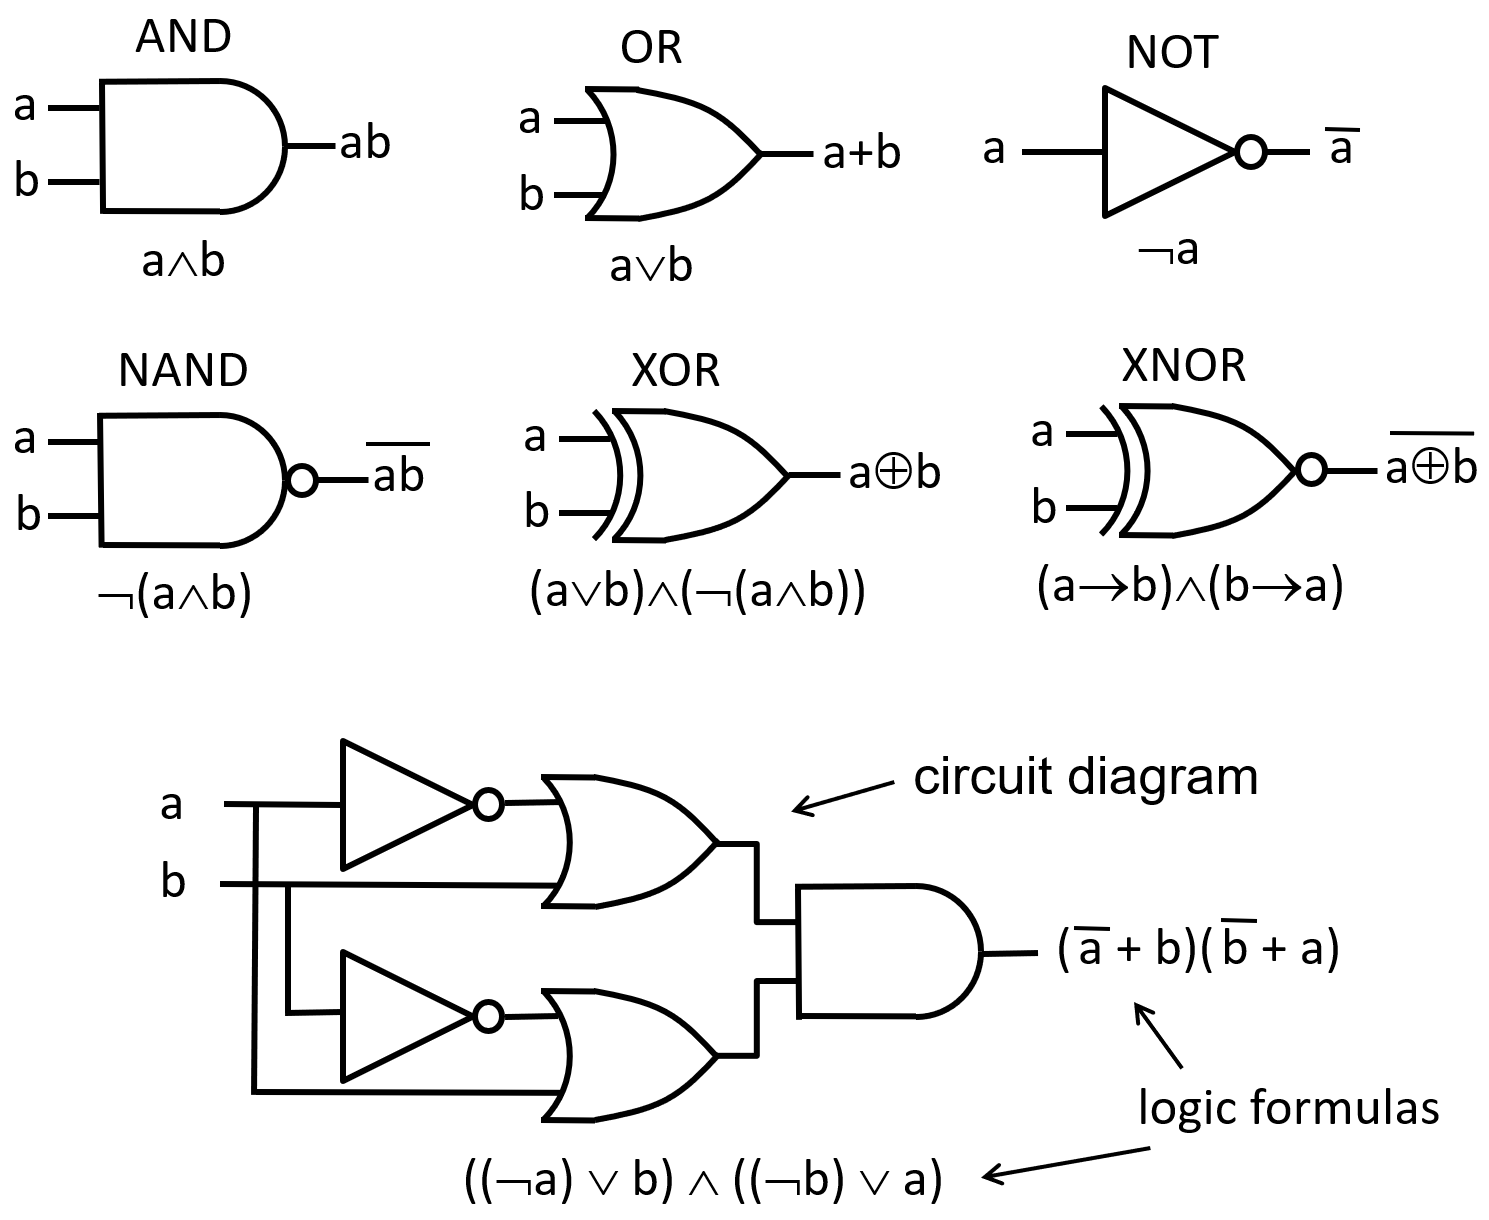
\includegraphics[scale=0.7]{Resources/LogicGates.png}
\todo{I did not have Visio with me. Improvised with PowerPoint. Figure will need to be redrawn.}
\end{center}
\caption{Digital Circuits = Logic Formulas}
\label{fig-02-logic-gates}
\end{figure}

Figure~\ref{fig-02-logic-gates} (see page \pageref{fig-02-logic-gates})
summarizes the relationships between
the symbols for logic gates in circuit diagrams (that is,
wiring diagrams that route signals between a collection of logic gates),
the algebraic notation used by circuit designers,
and the logic formulas we have used up to now.

The important fact to remember is this: All three notations
represent the same concepts in logic. Circuit diagrams, logic formulas,
and the algebraic notation used by circuit designers are three
different notations for exactly the same mathematical objects.
In this sense, digital circuits, and, therefore, computers,
are materializations of logic formulas. Computers truly are
``logic in action''.

The logical operators that we have been using are
logical-and, logical-or, implication, and negation.
These are sufficient to write formulas that have
any possible input/output relationship between the
variables in the formula and the value it delivers.

The \{implication\} axiom
(Figure~\ref{fig-02-boolean-axioms}, page \pageref{fig-02-boolean-axioms})
expresses implication in terms of logical-and, logical-or,
and negation, which means we lose no expressive power by
discarding implication from the set of logical operations.

Surprisingly, the reverse is also true.
That is, for any given input/output relationship that can be expressed
in a formula using logical-and, logical-or, and negation,
there is a logic formula using implication as
the only operator that has the same input/output relationship.
The \{$\neg$ as $\rightarrow$\} equation (see page \pageref{neg-as-imp})
provides at start in this direction by showing how to express
negation in terms of the implication operator.
Logical-and and logical-or are a little trickier.
You will will get a chance to look into that in the exercises
at the end of this section.

Furthermore, implication is not the only one-operator
basis for the entire system of logic. Another one
is the negation of logical-and, which is called ``nand''.

The nand gate is one of the standard logic gates,
and the fact that all of the other logical
operators can be expressed in terms of nand alone
makes the nand gate especially important.
It happens that the nand gate is the basis for designing most
large-scale digital circuits, such as computer chips.
Part of the reason for this is that the physics of putting gates on
chips is simplified when all of the gates are the same.

Let's see how nand can be a basis for the whole system.
We will express the operators in the basis we have at
this point ($\wedge$, $\vee$, and $\neg$) in terms of nand,
starting with negation.
Negation has only one input signals, and nand has two.
Feeding the same signal into both
inputs of a nand gate produces the behavior of
the negation operator.

It is easy to verify this from what we already know about logical operators
because there is a one-step proof of the following
equation. The proof cites the \{$\wedge$ idempotent\} theorem
(see page \pageref{and-idempotent}).

\begin{center}
\begin{tabular}{ll}
$(\neg a) = (\neg (a \wedge a))$  & \{$\neg$ as nand\}\label{neg-as-nand}
\end{tabular}
\end{center}

The \{$\neg$ as nand\} equation expresses negation
as a nand operation (the negation of a logical-and).
That takes care of negation. What about logical-and?

That's easy, too, because we only need to negate the
output from a nand gate, and we already know we can
use a nand gate to do that negation.
So, we can construct a circuit with the same behavior
as the logical-and by feeding the output signal
from one nand gate into both inputs of a second nand gate.

Algebraically, this circuit corresponds to the following equation.
It takes a two-step proof to verify the equation.
The first step converts the outside nand to negation using the
\{$\neg$ as nand\} equation, and the second step cites
the \{double negation\} axiom from Figure~\ref{fig-02-boolean-axioms}
(page \pageref{fig-02-boolean-axioms}).

\begin{center}
\begin{tabular}{ll}
$(a \wedge b) = (\neg ((\neg (a \wedge b)) \wedge (\neg (a \wedge b))))$ & \{$\wedge$ as nand\}\label{and-as-nand}
\end{tabular}
\end{center}

That takes care of logical-and, which brings us to logical-or.
Expressing logical-or in terms of nand is a little trickier
than the other two.
We got negation using one nand gate and
logical-and using two nand gates.
We will need three nand gates for logical-or,
and to verify the equation we will need a multi-step proof involving
the \{$\neg$ as nand\} equation, DeMorgan's laws,
and double negation.

\begin{center}
\begin{tabular}{ll}
$(a \vee b) = (\neg ((\neg(a \wedge a))) \wedge ((\neg(b \wedge b)))))$ & \{$\vee$ as nand\}\label{or-as-nand}
\end{tabular}
\end{center}

We will rely on you to carry out the proofs of the
\{$\neg$ as $\wedge$\}, \{$\wedge$ as nand\}, and \{$\vee$ as nand\} equations.
Figure~\ref{fig-02-nand-is-all-you-need} (page \pageref{fig-02-nand-is-all-you-need})
displays the digital circuits that
correspond to the equations verifying that nand is the only gate we really need.

\begin{figure}
\begin{center}
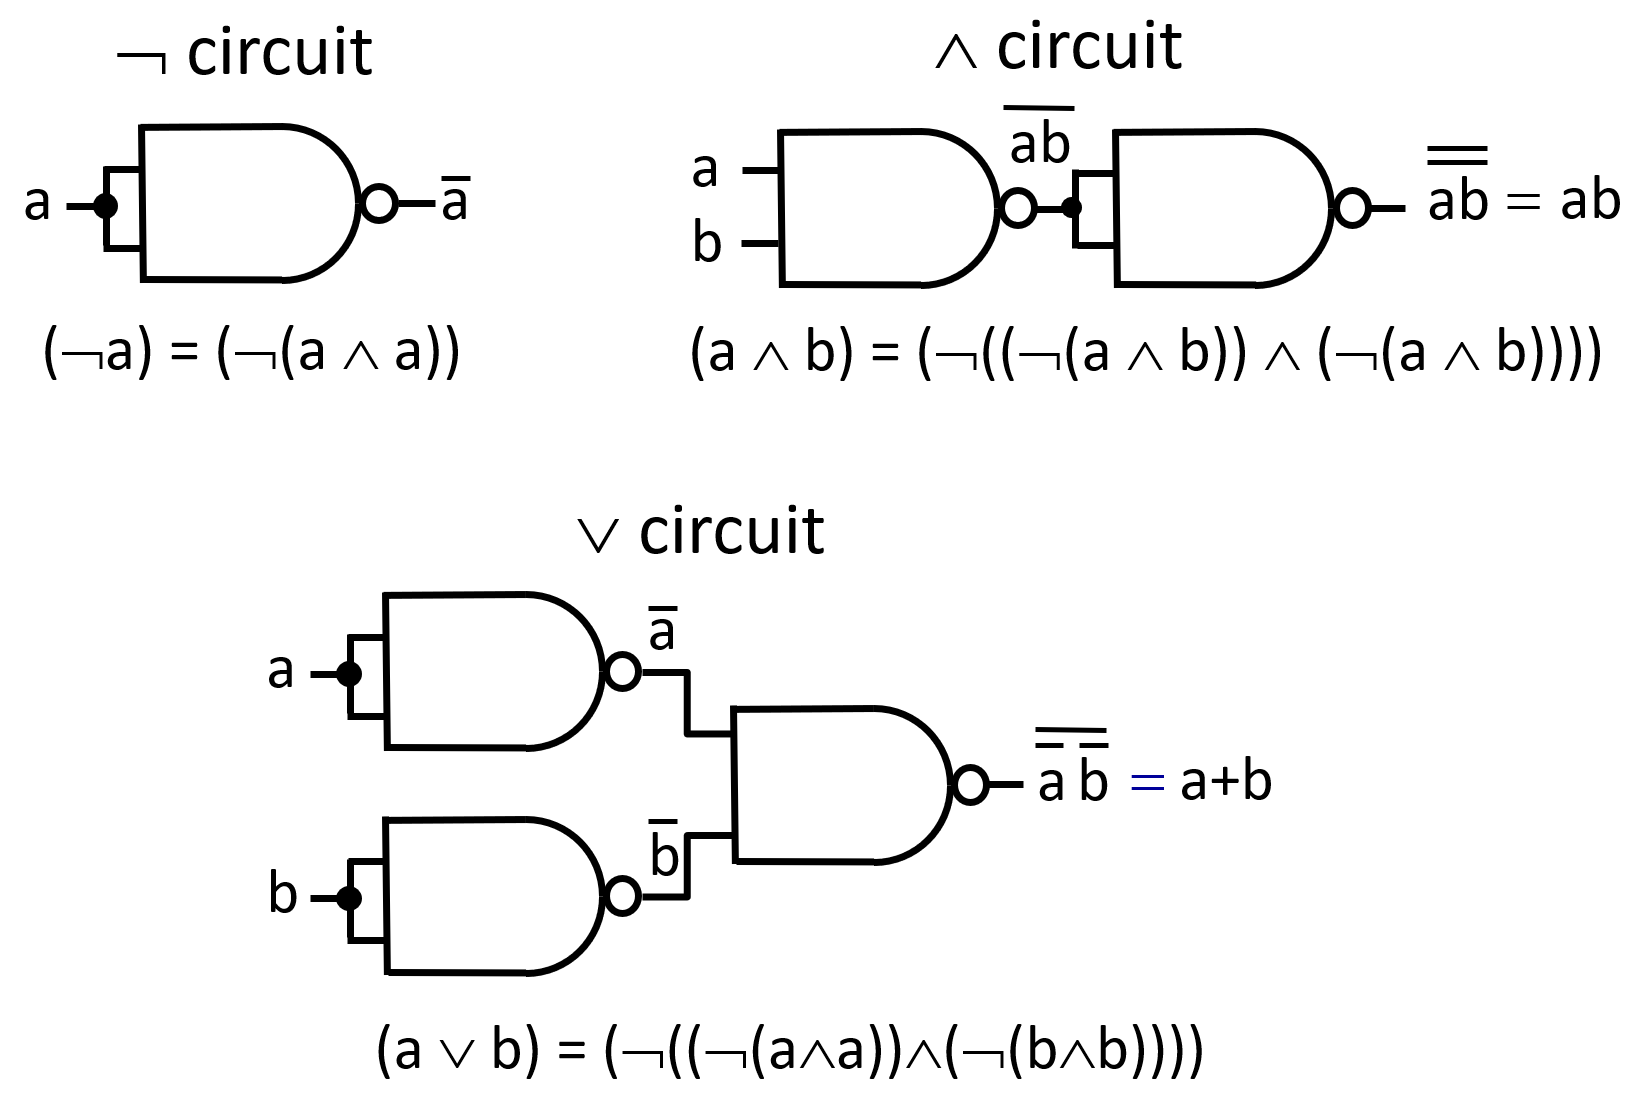
\includegraphics[scale=0.7]{Resources/NandIsAllYouNeed.png}
\todo{I did not have Visio with me. Improvised with PowerPoint. Figure will need to be redrawn.}
\end{center}
\caption{Nand is All You Need}
\label{fig-02-nand-is-all-you-need}
\end{figure}

\begin{ExerciseList}
\Exercise Using a negation-gate and an or-gate, draw a circuit diagram with the input/output behavior of the implication operator.
We refer to this circuit diagram as an ``implication circuit''.
Hint: Follow the example of the \{implication\} axiom
(Figure~\ref{fig-02-boolean-axioms}, page \pageref{fig-02-boolean-axioms})).
One of the inputs will need to be a constant rather than a variable.

\Exercise For each of the following logic formulas, draw an equivalent circuit diagram.
Since there are no ``implication operators'', they will need to be materialized
in the form of the circuit diagram from the previous exercise.
\begin{center}
\begin{tabular}{l}
$((a \vee (b \wedge (\neg a))) \vee (\neg (a \vee b)))$ \\
$(((\neg a) \wedge (\neg b)) \wedge (b \wedge (\neg c)))$ \\
$(a \rightarrow (b \rightarrow c))$ \\
$((a \wedge b) \rightarrow c)$ \\
\end{tabular}
\end{center}

\Exercise Rewrite each of the formulas in the previous exercise
in the algebraic notation used by electrical engineers:
juxtaposition for $\wedge$, + for $\vee$, and $\bar{a}$ for $(\neg a)$.

\Exercise Draw circuit diagrams with behavior of the and-gate, or-gate, and negation-gate,
but in these diagrams use implication circuits only---no other combinations of logic gates.
\end{ExerciseList}

\todo{ do we still want to add half-adder and/or full-adder
circuits as examples? problem: they have two outputs, so need to talk about
tapping outputs from subformulas to show correspondence to algebraic form}

\section{Deduction}

We have been reasoning with equations, which means we are reasoning in two directions
at the same time, since equations go both ways. Deductive reasoning is one-directional.
It derives a conclusion from hypotheses using one-directional rules of inference.
A proof shows that the conclusion is true whenever the hypotheses are true, but provides
no information about the conclusion when the truth of one or more of the hypotheses is
unknown.

Another way to say this is that a deductive proof of the formula $c$ (a conclusion)
from the formula $h$ (the hypothesis) guarantees that the formula
$(h \rightarrow c)$ is true.
Whenever we want to use deduction to prove that a formula with implication as its
top-level operator, $(h \rightarrow c)$, is true, this is the way we will do it.
We will construct a deductive proof of the conclusion $c$, assuming that
the hypothesis $h$ is true.

It is important to realize that proving an implication formula does
not require a proof of the hypothesis, only a derivation of the conclusion
from the hypothesis. This is because an implication formula is always
true if its hypothesis is false (by the \{$\rightarrow$ truth table\} theorem,
page \pageref{implication-truth-table}).
So, we can be sure that the implication formula is true as long as
we know that the only combination of values that makes the implication
$(h \rightarrow c)$ false, that is $h = True$ and $c = False$, cannot arise.

There might, of course, be any number of hypotheses, combined with
the $\wedge$ operator. If for example there are three hypotheses,
$h_1$, $h_2$, and $h_3$, then to use deduction to prove
$((h_1 \wedge h_2 \wedge h_3) \rightarrow c)$, we need to derive,
through the rules of deductive reasoning, the formula $c$ from
the formula $(h_1 \wedge h_2 \wedge h_3)$.

By the way, we have been a little cagey with the formula
$(h_1 \wedge h_2 \wedge h_3)$. It is not fully parenthesized.
Does it mean $((h_1 \wedge h_2) \wedge h_3)$ or
$(h_1 \wedge (h_2 \wedge h_3))$?
The answer is, it doesn't matter because of the \{$\wedge$ associative\}
theorem (page \pageref{and-associative}).
Both formulas have the same meaning.

There might even be no hypotheses at all, in which case a proof of the
conclusion $c$ would guarantee the truth of the formula
$c$. That is, the proof would guarantee the equation $c = True$.

We are not going to discuss deductive reasoning in great detail
because most of the things we will prove will come from reasoning
with equations. A formal treatment of deductive reasoning makes it
possible to prove all of the axioms of Boolean algebra
(Figure~\ref{fig-02-boolean-axioms}, page \pageref{fig-02-boolean-axioms})
from a small set of inference rules,
each of which is easily seen to be consistent with the use of logic in everyday life.

So, in a sense deductive reasoning gets closer to the fundamentals of
logic than the axioms of Boolean algebra, but we are more interested in getting at how
computers work than in building a formal system of logic from the ground up.
If you are interested in fundamentals, an accessible treatment can be found
in a text by O'Donnell, Hall, and Page
(\emph{Discrete Mathematics Using a Computer}, Springer, 2006).
See the sections on ``natural deduction'' (an invention of Gerhard Gentzen).

To give you a light introduction to how it works, consider the
rules of inference for deductive reasoning in Figure~\ref{fig-02-deduction-rules}
(page \pageref{fig-02-deduction-rules}).
One of the rules, \{$\rightarrow$ introduction\}, is a formal statement of the
discussion at the beginning of this section about proofs of implication formulas.

The \{$\vee$ elimination\} rule supports case-by-case proofs.
That is, if you can make a list of cases that covers all of the possibilities,
you can prove that a formula is true if you derive it from each of the
cases separately.

\begin{figure}
\begin{center}
\begin{tabular}{lllll}
Prove $a$                &                              &~~~~~& Prove $a \vee b$                   & \\
Prove $a \rightarrow b$  &                              &~~~~~& Prove $a \rightarrow c$            & \\
-----------------        &\{modus ponens\}              &~~~~~& Prove $b \rightarrow c$            & \\
Infer $b$                &                              &~~~~~& -----------------                  &\{$\vee$ elimination\} \\
                         &                              &~~~~~& Infer $c$                          & \\
                         &                              &~~~~~&                                    & \\
Prove $a$                &                              &~~~~~&                                    & \\
Prove $b$                &                              &~~~~~& Prove $(\neg a) \rightarrow False$ & \\
-----------              &\{$\wedge$ introduction\}     &~~~~~& ---------------------------        &\{reductio \\
Infer $a \wedge  b$      &                              &~~~~~& Infer $a$                          &~~~ad absurdum\} \\
                         &                              &~~~~~&                                    & \\
                         &                              &~~~~~&                                    & \\
Assume $a$               &                              &~~~~~& Prove $a \wedge b$                 & \\
Prove $b$                &                              &~~~~~& --------------                     &\{$\wedge$ elimination\} \\
-----------              &\{$\rightarrow$ introduction\}&~~~~~& Infer $a$                          & \\
Infer $a \rightarrow b$  &                              &~~~~~&                                    & \\
\end{tabular}
\end{center}
\caption{Rules of Inference for Reasoning by Deduction}
\label{fig-02-deduction-rules}
\end{figure}

The \{modus ponens\} rule, probably the most famous one because
of the well known ``Socrates was a man'' application, says that if you know that
the formula $a$ is true and that the formula $a \rightarrow b$ is true,
you can conclude that $b$ is true.

The \{reductio ad absurdum\} rule supports ``proof by contradiction''.
It says that if you can derive $False$
from $(\neg a)$, then $(\neg a)$ must be $False$, which means that $a$ must
be $True$.

The \{$\wedge$ elimination\} rule says that if you know $a \wedge b$,
you can conclude that $a$ must be $True$. The same goes for $b$ of
course, but that is another rule. We have not included it in the table because
our goal is to give you the general idea, not to put together a complete
set of rules. Following the approach we have stated here,
we would need to add five more rules
(the other version of \{$\wedge$ elimination\} being one of them)
to have a complete set that would allow us to derive all of the
equations of Boolean algebra.

Fortunately, citing equations from Boolean algebra to justify
steps is consistent with proof by deduction. That is, a formula
in a deductive proof may be replaced by an equivalent formula
justified by an equation known from Boolean algebra. So, if we
accept the \{$\wedge$ commutative\} equation (see page \pageref{and-commutative}),
we can derive the other \{$\wedge$ elimination\} from
Figure~\ref{fig-02-deduction-rules} (page \pageref{fig-02-deduction-rules}).

The rule would be stated as follows.
\begin{center}
\begin{tabular}{ll}
Prove $a \wedge b$                 & \\
--------------                     &\{$\wedge$ elimination-2\} \\
Infer $b$                          & \\
\end{tabular}
\end{center}

The derivation of the new rule, \{$\wedge$ elimination-2\},
proceeds by deductive reasoning as follows.
\begin{center}
\begin{tabular}{ll}
Prove $a \wedge b$                 & \\
--------------                     &\{$\wedge$ commutative\} \\
Prove $b \wedge a$                 & \\
--------------                     &\{$\wedge$ elimination\} \\
Infer $b$                          & \\
\end{tabular}
\end{center}

Just as with Boolean equations, once a new rule is proven, it
can be cited to justify steps in proofs.
So, at this point we could use \{$\wedge$ elimination-2\}
in a proof by deductive reasoning.

To firm up the idea at least a little,
we will do one more proof using deductive reasoning.
The theorem is known as the implication chain rule.

\begin{center}
\begin{tabular}{ll}
$((a \rightarrow b) \wedge (b \rightarrow c)) \rightarrow (a \rightarrow c)$ &\{$\rightarrow$ chain\}
\end{tabular}
\end{center}

The proof proceeds as follows.
\begin{center}
\begin{tabular}{ll}
Assume $((a \rightarrow b) \wedge (b \rightarrow c))$ & \\
------------------------------------                  &\{$\wedge$ elimination\} \\
Infer $(a \rightarrow b)$                             & \\
Assume $a$                                            & \\
------------------                                    &\{modus ponens\} \\
Infer $b$                                             & \\
Assume $((a \rightarrow b) \wedge (b \rightarrow c))$ & \\
------------------------------------                  &\{$\wedge$ elimination-2\} \\
Infer $(b \rightarrow c)$                             & \\
------------------                                    &\{modus ponens\} \\
Infer $c$                                             & \\
---------------                                       &\{$\rightarrow$ introduction\} \\
Infer ($a \rightarrow c$)                             & \\
------------------                                    &\{$\rightarrow$ introduction\} \\
Infer $((a \rightarrow b) \wedge (b \rightarrow c)) \rightarrow (a \rightarrow c)$ & \\
\end{tabular}
\end{center}

A tautology is a Boolean formula that has the value $True$ regardless of the values of its variables.
Put another way, a tautology is a Boolean formula that is equal to the formula $True$.

Every theorem proved by deduction confirms a tautology.
The tautological formula corresponding to a theorem is the implication with the logical-and
of the hypotheses as the operand on the left of the implication and the conclusion of the theorem
on the right. Since a tautology is a formula equal to $True$, every theorem leads to
a corresponding Boolean equation.

The \{$\rightarrow$ chain\} theorem that we just proved by deduction
confirms that the formula derived from the theorem in this way is equivalent to $True$.
In the form of an equation, this theorem would be stated as follows.
\begin{center}
\begin{tabular}{ll}
$(((a \rightarrow b) \wedge (b \rightarrow c)) \rightarrow (a \rightarrow c)) = True$ &\{$\rightarrow$ chain\}
\end{tabular}
\end{center}

If you want to get a little more practice in reasoning with equations,
construct a prooof of the \{$\rightarrow$ chain\} equation based on the
axioms of Boolean algebra (Figure~\ref{fig-02-boolean-axioms}, page \pageref{fig-02-boolean-axioms}).

\begin{ExerciseList}
\Exercise
Use the rules of inference for deduction (page \pageref{fig-02-deduction-rules})
to derive the formula $c$ from the formula
$(a \wedge ((a \rightarrow b) \wedge (b \rightarrow c)))$.

\Exercise
Use the axioms of Boolean algebra (page \pageref{fig-02-boolean-axioms})
to derive the equation
$((a \wedge ((a \rightarrow b) \wedge (b \rightarrow c))) \rightarrow c) = True$.

\Exercise
Explain the connection between the previous two exercises.
\end{ExerciseList}

\todo{Not sure whether we need a section on one-directional reasoning or not ...
seems like we do, but a full-fledged Gentzen-style treatment gets tedious ...
how do we keep it lively, but still provide the necessary apparatus? ...
Maybe better to introduce inference rules when we introduce induction? ...
how many rules do we need? Would modus ponens and or-elim (plus induction) be enough? How about reductio-ad-absurdum?
law of excluded middle? Just the rules we will be using in doing inductive proofs about software and circuits}
\todo{after writing this, I'm not sure it does any good.
I'm especially not sure the proof notation I've used is clearly explained.
I went through all the lectures, homeworks, and exams in the existing applied logic course, and did not find any theorems proved by deductive reasoning that were not more easily handled by stating them as implications and proving them as equations of the form $(a \rightarrow b) = True$.
I guess we could leave this stuff in, but give it short shrift, and refer back to it if necessary.
We will use deduction when we come to induction, which is a deductive inference rule, but
I'm not sure we need to make a big deal out of it}
\todo{Check to make sure predicates and quantifiers are covered somewhere.
Show how to convert between forall and exists.}

%%% Local Variables:
%%% mode: latex
%%% TeX-master: "book"
%%% End:
